\documentclass[11pt,a4paper]{article}

\usepackage[utf8]{inputenc}
\usepackage[T1]{fontenc}
\usepackage[brazil]{babel}
\usepackage[a4paper,margin=2.5cm]{geometry}
\usepackage{graphicx}
\usepackage{booktabs}
\usepackage{array}
\usepackage{url}
\usepackage{microtype}
\usepackage{amsmath}
\usepackage{tikz}
\usepackage{caption}
\usepackage[hidelinks]{hyperref}
\usetikzlibrary{arrows.meta,positioning,fit,calc}
\newcounter{algoritmo}

\emergencystretch=2em
\setlength{\parindent}{1.25cm}
\setlength{\parskip}{0pt}
\linespread{1.08}
\renewcommand{\abstractname}{Resumo}
\renewcommand{\refname}{Referências}
\captionsetup{font=small,labelfont=bf}

\title{Previsão Mensal de Irradiância Global Horizontal em Localidades de Fábricas de Veículos Elétricos com uma Aproximação do DeepNPTS}

\author{Gustavo de Melo Nascimento, Thales Wulfert Cabral e Gustavo Fraidenraich\\[0.4em]
\small Faculdade de Engenharia Elétrica e de Computação, Universidade Estadual de Campinas\\
\small Campinas, SP, Brasil\\
\small \texttt{g239679@dac.unicamp.br}, \texttt{t264377@dac.unicamp.br}, \texttt{gfraiden@unicamp.br}}
\date{}

\begin{document}

\maketitle

\begin{abstract}
Este artigo apresenta um sistema para previsão mensal da Irradiância Global Horizontal (GHI) em dez localidades associadas a fábricas de veículos elétricos. Foram utilizados dados da National Solar Radiation Database (NSRDB), mantida pelo atual National Laboratory of the Rockies (NLR, anteriormente NREL), produto GOES Aggregated PSM v4, no período de 2019 a 2024. Os dados, originalmente disponibilizados com resolução temporal de 60 minutos e consolidados pelo fluxo de processamento como médias diárias, foram agregados por mês civil, quantizados em 128 níveis, normalizados por min-max e organizados em atributos temporais para a previsão do mês seguinte. O método proposto é uma aproximação experimental inspirada no DeepNPTS e combina similaridade entre padrões históricos com ponderação por recência. A avaliação empregou uma divisão cronológica de 80\% para treinamento e 20\% para teste. Entre os sete modelos analisados, a aproximação proposta obteve o menor erro médio, com MAE de 12,96 W/m$^2$, RMSE de 16,39 W/m$^2$, $R^2$ de 0,916 e nRMSE de 8,10\%. Em comparação com a RNN, melhor modelo de referência em termos médios, o método reduziu o MAE em 12,50\% e o RMSE em 10,07\%.
\end{abstract}

\noindent\textbf{Palavras-chave:} irradiância solar; GHI; previsão mensal; séries temporais; DeepNPTS; aprendizado de máquina.

\section{Introdução}

A expansão da geração fotovoltaica aumenta a necessidade de estimar com antecedência a disponibilidade do recurso solar. Como a potência produzida por um sistema fotovoltaico depende diretamente da irradiância incidente, erros nessa estimativa afetam o dimensionamento de instalações, o planejamento da operação e a integração da geração à rede elétrica. Nesse contexto, a previsão de irradiância reduz a incerteza associada à fonte solar e fornece suporte quantitativo para decisões energéticas em diferentes horizontes temporais \cite{antonanzas2016,voyant2017,yang2018}.

Este trabalho utiliza a Irradiância Global Horizontal (GHI), isto é, a irradiância total recebida por uma superfície horizontal. Fisicamente, a GHI pode ser expressa pela Equação (\ref{eq:ghi}):

\begin{equation}
\mathrm{GHI}=\mathrm{DHI}+\mathrm{DNI}\cos(\theta_z),
\label{eq:ghi}
\end{equation}

\noindent em que DHI é a irradiância difusa horizontal, DNI é a irradiância direta normal e $\theta_z$ é o ângulo zenital solar \cite{duffie2013}. A escolha da GHI decorre de três características: ela representa conjuntamente as componentes direta e difusa, é disponibilizada de forma padronizada em bases de recurso solar e permite comparar localidades sob a mesma referência física, em W/m$^2$ \cite{sengupta2018}.

Em escala mensal, a previsão de GHI constitui um fator relevante para comparação de localidades, estimativa de produção, planejamento energético e avaliação preliminar de projetos fotovoltaicos. Diferentemente dos horizontes de minutos ou horas, fortemente influenciados por mudanças rápidas de nebulosidade, a agregação mensal ressalta a sazonalidade e as tendências de longo prazo do recurso solar \cite{antonanzas2016,voyant2022}. Essa agregação, entretanto, reduz substancialmente o número de observações: cada ano acrescenta somente doze amostras, o que torna a previsão mensal um problema de séries temporais curtas.

Métodos estatísticos, técnicas de aprendizado de máquina e redes neurais são empregados na previsão de irradiância \cite{sobri2018}. Neste estudo, XGBoost, Perceptron Multicamadas (MLP), Rede Neural Recorrente (RNN) e Long Short-Term Memory (LSTM) são utilizados como modelos de referência. O XGBoost representa relações não lineares por meio de árvores impulsionadas por gradiente \cite{chen2016}. As RNNs processam dependências sequenciais, enquanto a arquitetura LSTM foi desenvolvida para preservar informação ao longo de intervalos temporais mais extensos \cite{hochreiter1997}.

Avanços posteriores introduziram arquiteturas recorrentes multiescala, modelos probabilísticos e métodos não paramétricos. A DilatedRNN utiliza conexões recorrentes em diferentes resoluções temporais \cite{chang2017}, enquanto o DeepAR aprende distribuições preditivas por meio de uma rede recorrente autorregressiva \cite{salinas2017}. O Deep Non-Parametric Time Series Forecaster (DeepNPTS), por sua vez, aprende probabilidades de amostragem sobre observações históricas sem impor uma família paramétrica fixa à distribuição preditiva. Seus autores relatam desempenho consistente em bases com diferentes domínios e frequências \cite{rangapuram2023}. A capacidade de reutilizar padrões observados, mantendo as previsões relacionadas ao histórico da série, torna esse princípio particularmente atraente quando há poucas amostras mensais disponíveis.

Diante desse cenário, este trabalho propõe e avalia um sistema de previsão mensal de GHI baseado em uma aproximação experimental inspirada no DeepNPTS. O sistema processa séries de dez localidades associadas a fábricas de veículos elétricos, compara o método proposto com seis modelos concorrentes e seleciona o vencedor pelo menor erro absoluto médio (MAE) entre todas as localidades. A aproximação é adotada para investigar, de forma controlada, se a ponderação de padrões históricos por similaridade e recência pode produzir previsões robustas em séries mensais curtas.

\subsection{Principais contribuições}

As principais contribuições deste estudo são:

\begin{enumerate}
\renewcommand{\labelenumi}{(\roman{enumi})}
\item até onde foi possível verificar na literatura consultada, o primeiro estudo a empregar uma aproximação inspirada no DeepNPTS na previsão de GHI em escala mensal;
\item uma avaliação experimental em dez localidades, com comparação por localidade e por desempenho médio frente a modelos tabulares, recorrentes e probabilísticos; e
\item um fluxo reprodutível que integra aquisição, limpeza, agregação mensal, quantização, normalização, construção de atributos temporais, treinamento, avaliação e seleção pelo MAE médio.
\end{enumerate}

O restante do artigo está organizado da seguinte forma. A Seção \ref{sec:sistema} descreve o sistema proposto e seu algoritmo. A Seção \ref{sec:resultados} apresenta a configuração experimental, as métricas e a discussão dos resultados. Por fim, a Seção \ref{sec:conclusoes} reúne as conclusões, limitações e perspectivas de continuidade.

\section{Sistema proposto para previsão mensal de GHI}
\label{sec:sistema}

\subsection{Visão geral e fluxo de processamento}

A Figura \ref{fig:sistema_deepnpts} apresenta a visão geral do sistema proposto. O fluxo recebe séries de GHI associadas às localidades, aplica tratamento e transformação temporal, executa os modelos de IA e seleciona o método de menor MAE médio. Os estágios de (a) a (e) são descritos na mesma ordem em que aparecem na figura.

\begin{figure}[htbp]
\centering
\resizebox{\textwidth}{!}{%
\begin{tikzpicture}[
grupo/.style={draw, dashed, rounded corners=1pt, minimum height=3.8cm, inner sep=4pt},
caixa/.style={draw, align=center, minimum height=0.72cm, font=\scriptsize, fill=white},
titulo/.style={align=center, font=\scriptsize\bfseries},
rotulo/.style={font=\scriptsize},
seta/.style={-{Latex[length=2.2mm]}, thick}
]
\node[grupo, minimum width=2.55cm] (ga) at (0,0) {};
\node[titulo] at ([yshift=-0.35cm]ga.north) {Séries de GHI\\(dados brutos)};
\node[caixa, minimum width=1.75cm] (dados) at ([yshift=-1.85cm]ga.north) {$S_1$\\$S_2$\\$\vdots$\\$S_{|\mathcal L|}$};
\node[rotulo] at ([yshift=-0.28cm]ga.south) {(a)};

\node[grupo, minimum width=2.75cm] (gb) at (3.05,0) {};
\node[titulo] at ([yshift=-0.35cm]gb.north) {Tratamento inicial\\dos dados};
\node[caixa, minimum width=2.05cm] (limpeza) at ([yshift=-1.35cm]gb.north) {Limpeza de dados};
\node[caixa, minimum width=2.05cm, below=0.33cm of limpeza] (agrega) {Agregação\\mensal};
\draw[seta] (limpeza) -- (agrega);
\node[rotulo] at ([yshift=-0.28cm]gb.south) {(b)};

\node[grupo, minimum width=3.15cm] (gc) at (6.35,0) {};
\node[titulo] at ([yshift=-0.35cm]gc.north) {Pré-processamento e\\construção temporal};
\node[caixa, minimum width=2.4cm] (quant) at ([yshift=-1.20cm]gc.north) {Quantização};
\node[caixa, minimum width=2.4cm, below=0.23cm of quant] (norm) {Normalização min-max};
\node[caixa, minimum width=2.4cm, below=0.23cm of norm] (atrib) {Defasagens e médias móveis};
\draw[seta] (quant) -- (norm);
\draw[seta] (norm) -- (atrib);
\node[rotulo] at ([yshift=-0.28cm]gc.south) {(c)};

\node[grupo, minimum width=3.45cm] (gd) at (10.15,0) {};
\node[titulo] at ([yshift=-0.35cm]gd.north) {Estágio de previsão\\modelos de IA};
\node[caixa, minimum width=2.65cm, fill=green!8] (modelos) at ([yshift=-1.85cm]gd.north) {DeepNPTS (aprox.)\\\textit{versus}\\XGBoost, MLP, RNN, LSTM,\\DilatedRNN exp. e DeepAR exp.};
\node[rotulo] at ([yshift=-0.28cm]gd.south) {(d)};

\node[grupo, minimum width=3.25cm] (ge) at (13.95,0) {};
\node[titulo] at ([yshift=-0.35cm]ge.north) {Avaliação e\\seleção};
\node[caixa, minimum width=2.45cm] (pred) at ([yshift=-1.15cm]ge.north) {Previsões mensais};
\node[caixa, minimum width=2.45cm, below=0.23cm of pred] (metricas) {Métricas por localidade};
\node[caixa, minimum width=2.45cm, below=0.23cm of metricas, fill=orange!10] (campeao) {$\overline{\mathrm{MAE}}_{m}$\\modelo campeão};
\draw[seta] (pred) -- (metricas);
\draw[seta] (metricas) -- (campeao);
\node[rotulo] at ([yshift=-0.28cm]ge.south) {(e)};

\draw[seta] (dados.east) -- (limpeza.west);
\draw[seta] (agrega.east) -- (quant.west);
\draw[seta] (atrib.east) -- (modelos.west);
\draw[seta] (modelos.east) -- (pred.west);
\end{tikzpicture}%
}
\caption{Visão geral do sistema proposto para previsão mensal de GHI. O sistema inicia em (a) com as séries de GHI das localidades. Em seguida, (b) realiza limpeza e agregação mensal. O estágio (c) aplica quantização, normalização min-max e constrói os atributos temporais. Depois, (d) executa a aproximação do DeepNPTS e os modelos concorrentes. Finalmente, (e) calcula as métricas por localidade, obtém o MAE médio e determina o modelo campeão.}
\label{fig:sistema_deepnpts}
\end{figure}

\noindent\textbf{\textit{Estágio (a) -- séries de GHI.}} Para cada localidade $\ell\in\mathcal L$, a coleta produz uma série $S_{\ell}$ de GHI e preserva data, coordenadas e produto de origem. A GHI é mantida em W/m$^2$, permitindo comparar todas as fábricas sob a mesma grandeza física \cite{sengupta2018}.

\noindent\textbf{\textit{Estágio (b) -- tratamento inicial.}} Cada série é ordenada e examinada quanto à cobertura temporal, duplicidades, ausências, valores negativos e consistência geográfica. As observações diárias validadas são então agrupadas por mês civil por meio da média aritmética.

\noindent\textbf{\textit{Estágio (c) -- pré-processamento.}} A GHI mensal é quantizada e normalizada por min-max. Os limites da transformação são estimados apenas no treinamento e reutilizados no teste. Defasagens e médias móveis formam os pares supervisionados $(X_{\ell},y_{\ell})$, em que $y_{\ell}$ representa a GHI do mês seguinte.

\subsection{Aproximação inspirada no DeepNPTS}

\noindent\textbf{\textit{Estágio (d) -- modelos de IA.}} Os conjuntos temporais alimentam a aproximação do DeepNPTS, XGBoost, MLP, RNN, LSTM e as implementações experimentais de DilatedRNN e DeepAR. A Figura \ref{fig:deepnpts_interno} detalha o método proposto: o vetor corrente e os históricos candidatos determinam pesos de similaridade e recência, posteriormente combinados para produzir a previsão. Essa construção é inspirada no princípio não paramétrico de Rangapuram et al. \cite{rangapuram2023}, que reutiliza observações históricas para formar a distribuição preditiva.

\begin{figure}[htbp]
\centering
\resizebox{0.72\textwidth}{!}{%
\begin{tikzpicture}[
caixa/.style={draw, align=center, minimum height=0.78cm, minimum width=1.62cm, font=\scriptsize},
seta/.style={-{Latex[length=2mm]}, thick},
node distance=0.32cm
]
\node[caixa] (entrada) {Vetor atual\\$X_{\ell,t}$};
\node[caixa, below=0.38cm of entrada] (hist) {Históricos\\$\mathcal H_{\ell,t}$};
\node[caixa, right=0.55cm of entrada, yshift=-0.58cm] (pesos) {Similaridade $d$\\+ recência $\gamma$};
\node[caixa, right=of pesos] (normp) {Pesos\\$w_{t,j}$};
\node[caixa, right=of normp, fill=green!8] (saida) {Previsão\\$\hat y_{\ell,t+1}$};
\draw[seta] (entrada.east) -- (pesos.west);
\draw[seta] (hist.east) -- (pesos.west);
\draw[seta] (pesos) -- (normp);
\draw[seta] (normp) -- (saida);
\end{tikzpicture}%
}
\caption{Estrutura da aproximação do DeepNPTS. O vetor atual e os históricos alimentam o cálculo de similaridade e recência; os pesos resultantes produzem a previsão mensal ponderada.}
\label{fig:deepnpts_interno}
\end{figure}

A previsão pontual ilustrada na Figura \ref{fig:deepnpts_interno} é calculada por

\begin{equation}
\begin{aligned}
\hat{y}_{\ell,t+1}
&=\frac{\sum_{j\in\mathcal{H}_{\ell,t}}w_{t,j}y_{\ell,j+1}}
{\sum_{j\in\mathcal{H}_{\ell,t}}w_{t,j}},\\
w_{t,j}
&=\exp\!\left[-d(X_{\ell,t},X_{\ell,j})/\tau\right]\gamma^{t-j},
\end{aligned}
\label{eq:deepnpts}
\end{equation}

em que $\mathcal H_{\ell,t}$ é o conjunto de históricos candidatos, $d(\cdot)$ é a distância euclidiana entre vetores, $\tau$ controla a concentração dos pesos e $\gamma$ controla a recência. Diferentemente do DeepNPTS canônico, a implementação avaliada não treina uma rede global nem otimiza o escore de probabilidade ranqueado: ela calcula diretamente os pesos da Equação (\ref{eq:deepnpts}) em cada série. Para concisão, o rótulo ``DeepNPTS'' nas tabelas e figuras designa essa aproximação experimental, e não uma reprodução integral da arquitetura original.

\subsection{Critério de seleção e pseudocódigo}

\noindent\textbf{\textit{Estágio (e) -- avaliação e seleção.}} Cada modelo $m$ gera previsões $\hat y_{\ell,m}$ na escala física. Em seguida, o sistema calcula as métricas em cada localidade e obtém o MAE médio

\begin{equation}
\begin{aligned}
\overline{\mathrm{MAE}}_{m}&=\frac{1}{|\mathcal{L}|}\sum_{\ell\in\mathcal{L}}\mathrm{MAE}_{\ell,m},\\
m^{\star}&=\underset{m\in\mathcal{M}}{\arg\min}\ \overline{\mathrm{MAE}}_{m}.
\end{aligned}
\label{eq:selecao}
\end{equation}

Assim, $m^{\star}$ é o modelo de menor MAE médio entre todas as fábricas, mesmo que outro método seja superior em uma localidade isolada. O Algoritmo \ref{alg:sistema} formaliza esse fluxo sem fixar valores numéricos.

\begin{figure}[htbp]
\centering
\refstepcounter{algoritmo}\label{alg:sistema}
\textbf{Algoritmo \thealgoritmo: Previsão e seleção do modelo}

\fbox{%
\begin{minipage}{0.90\textwidth}
\footnotesize
\begin{tabbing}
\quad\=\quad\=\kill
\textbf{Entrada:} séries $\mathcal S$, localidades $\mathcal L$, modelos $\mathcal M$,\\
\> horizonte $h$ e proporção $\rho$.\\
\textbf{Para cada} $\ell\in\mathcal L$ \textbf{faça}\\
\> $S_{\ell}\leftarrow$ coletar, limpar e agregar a série;\\
\> $c_{\ell}\leftarrow$ determinar o corte cronológico por $\rho$;\\
\> $q_{\ell}\leftarrow$ ajustar quantização e normalização antes de $c_{\ell}$;\\
\> $Z_{\ell}\leftarrow$ transformar $S_{\ell}$ com $q_{\ell}$;\\
\> $(X_{\ell},y_{\ell})\leftarrow$ construir atributos e alvo $h$;\\
\> $(D_{\ell}^{tr},D_{\ell}^{te})\leftarrow$ dividir temporalmente em $c_{\ell}$;\\
\> \textbf{Para cada} $m\in\mathcal M$ \textbf{faça}\\
\>\> $f_{\ell,m}\leftarrow$ treinar $m$ em $D_{\ell}^{tr}$;\\
\>\> $\hat y_{\ell,m}\leftarrow f_{\ell,m}(D_{\ell}^{te})$;\\
\>\> $E_{\ell,m}\leftarrow$ avaliar $(y_{\ell}^{te},\hat y_{\ell,m})$;\\
\> \textbf{fim}\\
\textbf{fim}\\
$m^{\star}\leftarrow\arg\min_{m\in\mathcal M}\overline{\mathrm{MAE}}_{m}$;\\
\textbf{Saída:} $m^{\star}$, previsões e métricas.
\end{tabbing}
\end{minipage}}
\end{figure}

No Algoritmo \ref{alg:sistema}, as primeiras operações reproduzem os estágios (a)--(c) da Figura \ref{fig:sistema_deepnpts}; o laço interno corresponde ao estágio (d); e o cálculo de $m^{\star}$ implementa o estágio (e). Desse modo, diagrama, formulação matemática e pseudocódigo descrevem o mesmo procedimento experimental.

\section{Resultados e discussão}
\label{sec:resultados}

Esta seção descreve inicialmente a base de dados, a configuração dos modelos e as métricas de avaliação. Em seguida, os resultados são analisados em três níveis: desempenho médio entre localidades, desempenho específico por localidade e aderência das previsões à série temporal de teste.

\subsection{Base de dados e configuração experimental}

A avaliação utiliza GHI da NSRDB, atualmente disponibilizada pelo NLR (antigo NREL), para dez localidades: BYD Camaçari, BMW San Luis Potosí, Ford Rouge, GM Factory Zero, Hyundai Metaplant Georgia, Lucid AMP 1 Casa Grande, Rivian Normal e as unidades Tesla de Fremont, Nevada e Texas. A consulta empregou o produto GOES Aggregated PSM v4 e cobre o período de 1 de janeiro de 2019 a 31 de dezembro de 2024 \cite{nlr2026}.

A API foi consultada em intervalos de 60 minutos; o fluxo de processamento armazenou médias diárias, posteriormente agregadas por mês civil. Após a criação das variáveis temporais, cada localidade fornece 60 exemplos supervisionados, com alvos entre janeiro de 2020 e dezembro de 2024: 48 exemplos são destinados ao treinamento e 12 ao teste, estes correspondentes aos meses de 2024. O protocolo é de previsão direta de um mês à frente. Em cada exemplo de teste, os atributos utilizam somente observações disponíveis até o mês corrente para estimar o mês seguinte; os modelos permanecem fixos, sem novo ajuste durante o teste. A Tabela \ref{tab:configuracao} reúne as condições de avaliação.

\begin{table}[htbp]
\centering
\caption{Configurações da avaliação experimental.}
\label{tab:configuracao}
\begingroup
\small
\setlength{\tabcolsep}{4pt}
\renewcommand{\arraystretch}{1.06}
\begin{tabular}{>{\raggedright\arraybackslash}p{3.8cm}>{\raggedright\arraybackslash}p{10.8cm}}
\toprule
\textbf{Item} & \textbf{Configuração utilizada} \\
\midrule
Fonte dos dados & NSRDB/NLR (antigo NREL), produto GOES Aggregated PSM v4. \\
Grandeza analisada & GHI em W/m$^2$. \\
Frequência de coleta & 60 minutos na API; arquivo processado como média diária; agregação final mensal. \\
Período de coleta & 2019 a 2024. \\
Horizonte de previsão & Um mês à frente. \\
Particionamento & Divisão cronológica 80\%/20\%, sem embaralhamento: 48 exemplos de treino e 12 de teste por localidade. \\
Procedimento de teste & Doze previsões diretas e sucessivas de um mês à frente, sem retreinamento; cada entrada contém apenas o histórico disponível até o instante da previsão. \\
Pré-processamento & Quantização em 128 níveis e normalização min-max ajustadas no treino; defasagens de 1, 2, 3 e 6 meses; médias móveis de 3, 6 e 12 meses. \\
Ambiente disponível para reprodução & Linux 6.8, Python 3.12.1, 2 vCPUs AMD EPYC 9V74, 7,8 GiB de RAM e sem GPU NVIDIA detectada. \\
\bottomrule
\end{tabular}
\endgroup
\end{table}

Os arquivos do projeto não registram o hardware original de todas as execuções; por isso, a Tabela \ref{tab:configuracao} informa o ambiente atualmente disponível para reprodução, sem atribuí-lo retroativamente aos treinamentos.

\subsection{Modelos e hiperparâmetros}

Os hiperparâmetros efetivamente registrados estão resumidos na Tabela \ref{tab:hiperparametros}. A mesma divisão temporal e as mesmas sete variáveis de entrada foram empregadas para tornar a comparação entre os modelos consistente. Nos métodos estocásticos, adotou-se a semente 42.

\begin{table}[htbp]
\centering
\caption{Hiperparâmetros dos modelos avaliados.}
\label{tab:hiperparametros}
\begingroup
\small
\setlength{\tabcolsep}{4pt}
\renewcommand{\arraystretch}{1.06}
\begin{tabular}{>{\raggedright\arraybackslash}p{2.8cm}>{\raggedright\arraybackslash}p{11.8cm}}
\toprule
\textbf{Modelo} & \textbf{Configuração} \\
\midrule
XGBoost & 300 estimadores, profundidade máxima 3, taxa de aprendizagem 0,05, \textit{subsample} 0,9, \textit{colsample} 0,9, objetivo \textit{squarederror}. \\
MLP & Camadas ocultas 64 e 32, ativação ReLU, Adam, taxa inicial 0,001, máximo de 1000 iterações. \\
RNN & SimpleRNN com 32 unidades, camada densa de 16 neurônios ReLU, saída sigmoidal, MSE, Adam 0,001, 80 épocas e lote 32. \\
LSTM & LSTM com 32 unidades, camada densa de 16 neurônios ReLU, saída sigmoidal, MSE, Adam 0,001, 80 épocas e lote 32. \\
DilatedRNN exp. & Três ramos recorrentes com dilatações 1, 2 e 4, 32 unidades por ramo, densa de 16 neurônios, MSE, Adam 0,001, 80 épocas e lote 32. \\
DeepAR exp. & LSTM probabilística com 32 unidades, saída de média e dispersão, perda gaussiana, Adam 0,001, 80 épocas e lote 32. \\
DeepNPTS aprox. & $k=80$ (limitado aos 48 exemplos de treino), temperatura 0,08 e decaimento de recência 0,995. \\
\bottomrule
\end{tabular}
\endgroup
\end{table}

Como cada conjunto de treinamento contém 48 exemplos, o critério de ativação da validação interna, definido para pelo menos 50 exemplos, não foi alcançado. Assim, RNN, LSTM, DilatedRNN e DeepAR executaram as 80 épocas, sem parada antecipada. Os resultados correspondem a uma execução por modelo e localidade com a semente especificada.

\subsection{Métricas de avaliação}

As métricas cobrem cinco aspectos complementares: magnitude absoluta do erro, penalização de desvios elevados, erro na unidade original, variabilidade explicada e erro relativo. Essa combinação evita que a análise dependa de uma única propriedade estatística \cite{hyndman2006,voyant2022}. Sejam $y_i$ a GHI real em W/m$^2$, $\hat{y}_i$ a previsão na mesma unidade, $\bar{y}$ a média das observações e $n$ o número de amostras de teste. As métricas são

\begin{align}
\mathrm{MAE} &= \frac{1}{n}\sum_{i=1}^{n}|y_i-\hat{y}_i|, \label{eq:mae}\\
\mathrm{MSE} &= \frac{1}{n}\sum_{i=1}^{n}(y_i-\hat{y}_i)^2, \label{eq:mse}\\
\mathrm{RMSE} &= \sqrt{\frac{1}{n}\sum_{i=1}^{n}(y_i-\hat{y}_i)^2}, \label{eq:rmse}\\
R^2 &= 1-\frac{\sum_{i=1}^{n}(y_i-\hat{y}_i)^2}{\sum_{i=1}^{n}(y_i-\bar{y})^2}, \label{eq:r2}\\
\mathrm{nRMSE}(\%) &= 100\frac{\mathrm{RMSE}}{\bar{y}}. \label{eq:nrmse}
\end{align}

O MAE da Equação (\ref{eq:mae}) é diretamente interpretável em W/m$^2$ e, por isso, define o modelo vencedor. O MSE da Equação (\ref{eq:mse}) enfatiza erros grandes e é expresso em W$^2$/m$^4$. O RMSE da Equação (\ref{eq:rmse}) preserva essa sensibilidade e retorna a W/m$^2$. O $R^2$ da Equação (\ref{eq:r2}) é adimensional e mede a variabilidade explicada em relação à média, enquanto o nRMSE da Equação (\ref{eq:nrmse}) expressa o RMSE como porcentagem da GHI média e facilita comparações entre localidades.

\subsection{Comparação média entre os modelos}

A primeira questão experimental consiste em identificar o modelo com desempenho mais consistente no conjunto das dez localidades. Para respondê-la, a Tabela \ref{tab:metricas_medias} reúne as médias das métricas. Os modelos estão ordenados pelo MAE, conforme o critério de seleção definido na Equação (\ref{eq:selecao}).

\begin{table}[htbp]
\centering
\caption{Métricas médias mensais dos modelos avaliados.}
\label{tab:metricas_medias}
\small
\resizebox{0.92\textwidth}{!}{%
\begin{tabular}{lrrrrr}
\toprule
\textbf{Modelo} & \textbf{MAE} & \textbf{MSE} & \textbf{RMSE} & \textbf{R$^2$} & \textbf{nRMSE} \\
 & \textbf{W/m$^2$} & \textbf{W$^2$/m$^4$} & \textbf{W/m$^2$} & & \textbf{\%} \\
\midrule
DeepNPTS aprox. & 12,96 & 281,29 & 16,39 & 0,916 & 8,10 \\
RNN & 14,81 & 363,32 & 18,23 & 0,878 & 8,97 \\
XGBoost & 15,23 & 415,07 & 19,41 & 0,875 & 9,70 \\
DilatedRNN exp. & 15,25 & 380,90 & 18,73 & 0,878 & 9,29 \\
MLP & 16,13 & 412,61 & 19,70 & 0,861 & 9,58 \\
LSTM & 20,60 & 659,72 & 24,69 & 0,785 & 11,99 \\
DeepAR exp. & 61,02 & 5038,27 & 68,57 & 0,010 & 34,21 \\
\bottomrule
\end{tabular}%
}
\end{table}

Como representação visual do ranqueamento, a Figura \ref{fig:mae_medio} apresenta o MAE médio de cada modelo. A diferença entre o grupo principal e o DeepAR experimental indica que a configuração probabilística utilizada não se ajustou adequadamente às séries mensais curtas.

\begin{figure}[htbp]
\centering
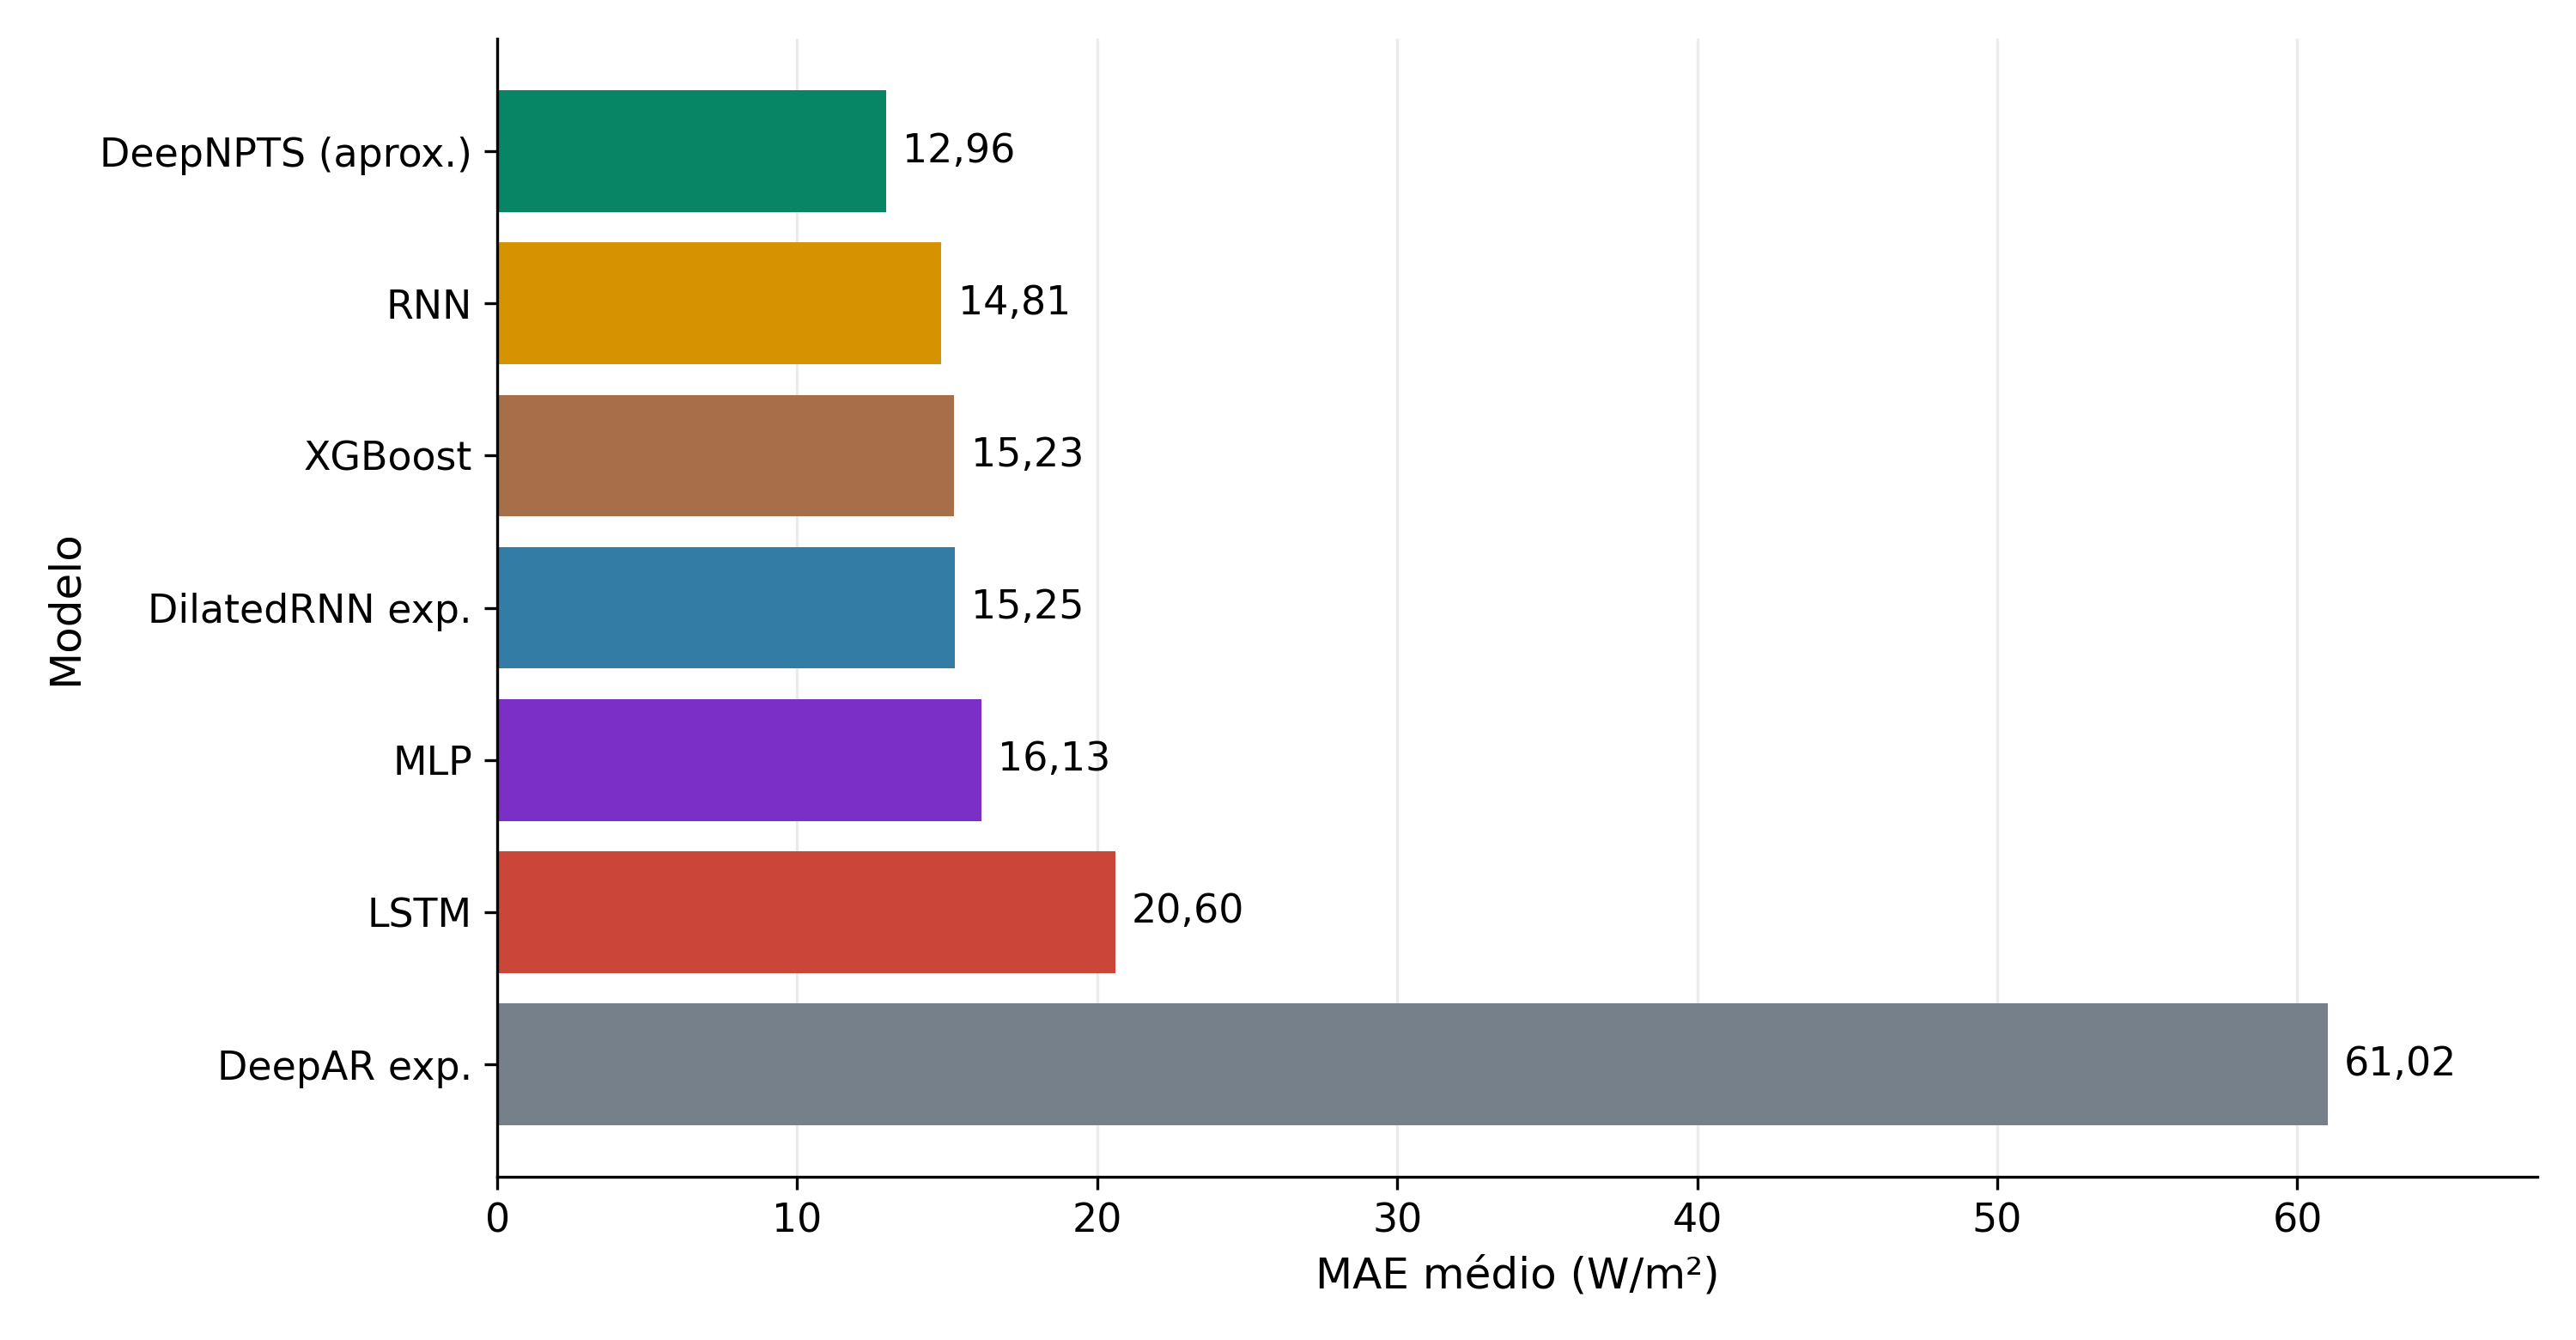
\includegraphics[width=0.88\textwidth]{figuras/mae_medio_modelos.png}
\caption{MAE médio dos modelos nas dez localidades; valores menores indicam melhor desempenho. O rótulo DeepNPTS corresponde à aproximação experimental.}
\label{fig:mae_medio}
\end{figure}

A Tabela \ref{tab:metricas_medias} e a Figura \ref{fig:mae_medio} apontam a aproximação do DeepNPTS como campeã geral. Em relação à RNN, melhor modelo de referência em termos médios, o MAE diminuiu de 14,81 para 12,96 W/m$^2$, o que representa uma redução de 12,50\%. O RMSE foi reduzido em 10,07\%. Em comparação com o DeepAR experimental, pior resultado médio, a redução do MAE foi de 78,76\%. A aproximação também alcançou o maior $R^2$ médio e o menor nRMSE, indicando que sua vantagem não depende exclusivamente da métrica utilizada para a seleção.

\subsection{Análise por localidade}

A média geral pode ocultar diferenças regionais. Por essa razão, a Tabela \ref{tab:deepnpts_localidades} apresenta todas as métricas da aproximação do DeepNPTS no teste mensal, enquanto a Figura \ref{fig:mae_localidades} compara seu MAE ao melhor concorrente de cada localidade.

\begin{table}[htbp]
\centering
\caption{Desempenho da aproximação do DeepNPTS por localidade no conjunto de teste.}
\label{tab:deepnpts_localidades}
\small
\resizebox{0.96\textwidth}{!}{%
\begin{tabular}{lrrrrr}
\toprule
\textbf{Localidade} & \textbf{MAE} & \textbf{MSE} & \textbf{RMSE} & \textbf{$R^2$} & \textbf{nRMSE} \\
 & \textbf{W/m$^2$} & \textbf{W$^2$/m$^4$} & \textbf{W/m$^2$} & & \textbf{\%} \\
\midrule
BMW S. L. Potosí & 18,65 & 528,90 & 23,00 & 0,738 & 9,28 \\
BYD Camaçari & 13,85 & 311,18 & 17,64 & 0,778 & 7,47 \\
Ford Rouge & 13,21 & 265,54 & 16,30 & 0,956 & 10,16 \\
GM Factory Zero & 13,24 & 300,51 & 17,34 & 0,949 & 10,82 \\
Hyundai Georgia & 11,25 & 189,33 & 13,76 & 0,937 & 6,94 \\
Lucid Casa Grande & 10,40 & 152,73 & 12,36 & 0,972 & 5,01 \\
Rivian Normal & 18,41 & 481,17 & 21,94 & 0,918 & 12,19 \\
Tesla Fremont & 10,83 & 237,67 & 15,42 & 0,973 & 6,99 \\
Tesla Nevada & 10,24 & 205,82 & 14,35 & 0,977 & 6,46 \\
Tesla Texas & 9,50 & 140,10 & 11,84 & 0,958 & 5,67 \\
\bottomrule
\end{tabular}%
}
\end{table}

\begin{figure}[htbp]
\centering
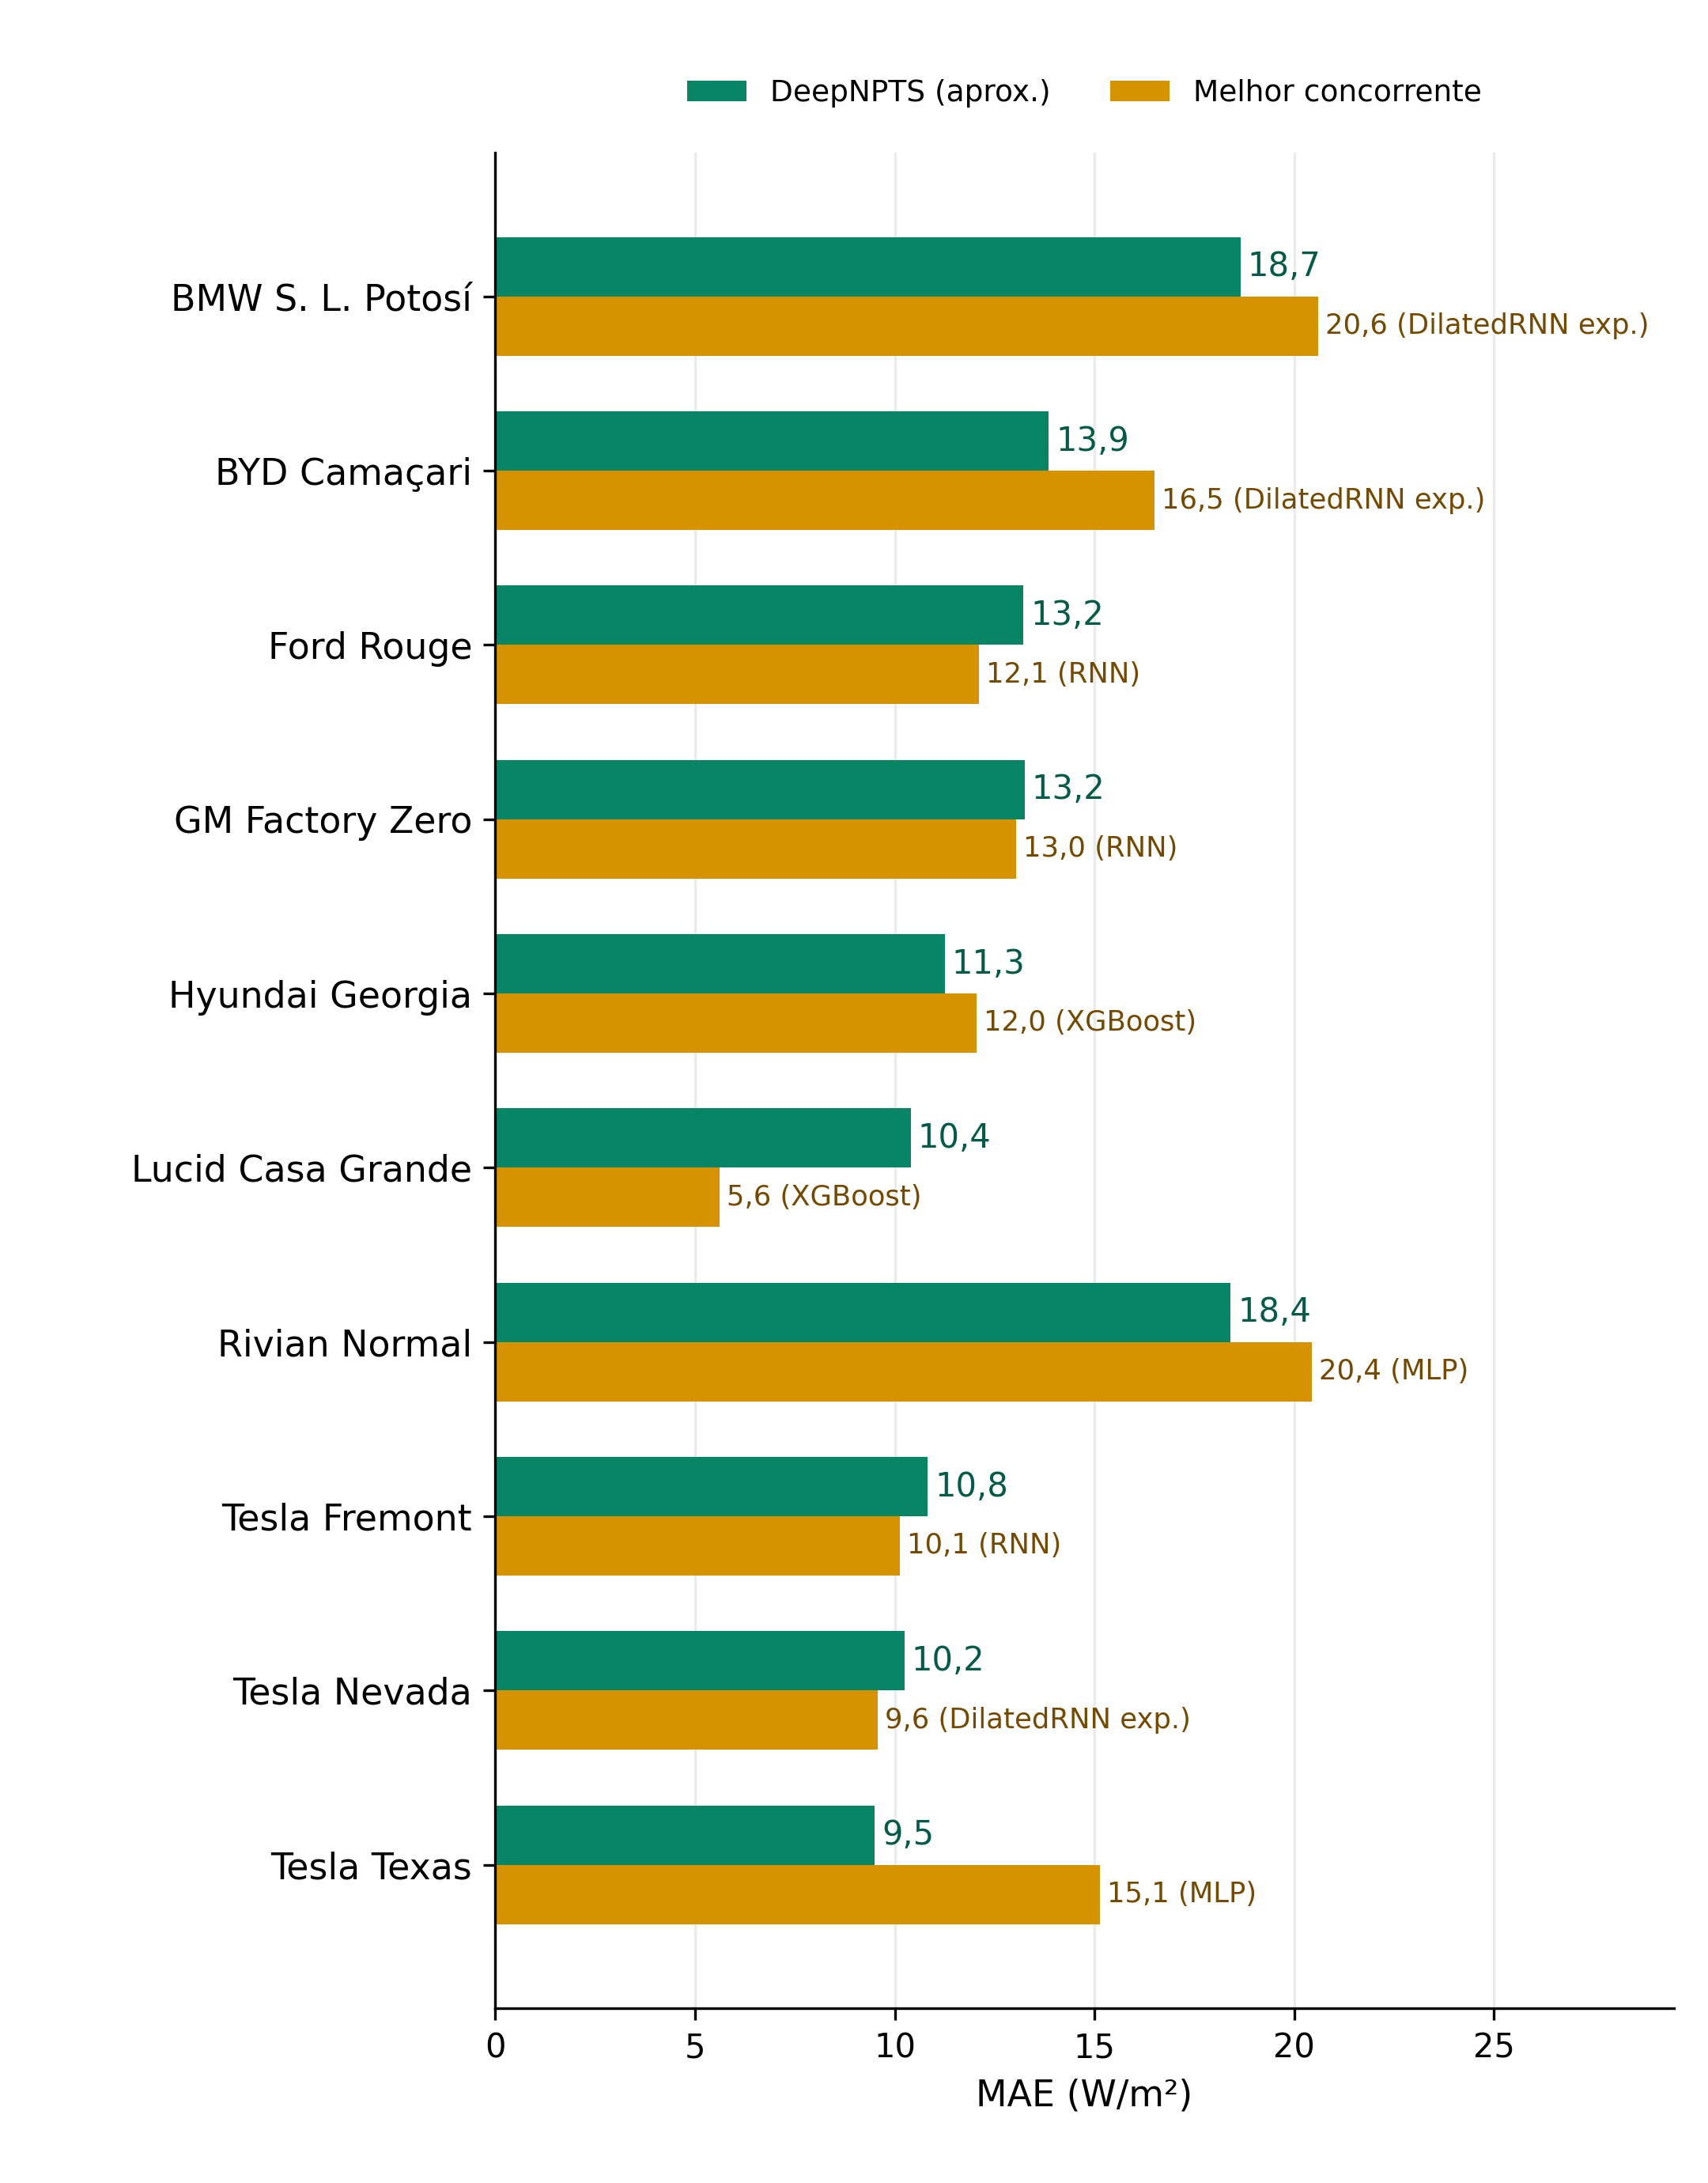
\includegraphics[width=0.68\textwidth]{figuras/mae_deepnpts_por_localidade_coluna.png}
\caption{MAE da aproximação do DeepNPTS e do melhor concorrente em cada localidade. As barras verdes representam o método proposto, e as barras amarelas identificam o concorrente de menor MAE.}
\label{fig:mae_localidades}
\end{figure}

Usando o menor MAE em cada localidade como critério, a aproximação do DeepNPTS venceu em cinco das dez localidades: BMW San Luis Potosí, BYD Camaçari, Hyundai Metaplant Georgia, Rivian Normal e Tesla Gigafactory Texas. A RNN venceu em três localidades: Ford Rouge Electric Vehicle Center, GM Factory Zero e Tesla Fremont Factory. O XGBoost venceu em Lucid AMP 1 Casa Grande, e a DilatedRNN experimental venceu em Tesla Gigafactory Nevada.

O melhor MAE da aproximação ocorreu na Tesla Texas (9,50 W/m$^2$), e o pior, na BMW San Luis Potosí (18,65 W/m$^2$). A diferença entre esses extremos foi de 9,15 W/m$^2$, equivalente a 49,1\% do pior resultado. Na Tesla Texas, a redução em relação à MLP, melhor concorrente local, foi de 37,23\%. Em contraste, o XGBoost venceu com margem expressiva na Lucid Casa Grande: 5,61 contra 10,40 W/m$^2$. A Figura \ref{fig:mae_localidades} mostra, portanto, que o método proposto é robusto em média, mas não domina uniformemente todas as condições regionais.

\subsection{Análise da previsão ao longo do tempo}

Além das métricas agregadas, é importante verificar se as previsões acompanham a forma da série observada. A Figura \ref{fig:previsao_byd} confronta a GHI real com as previsões da RNN, melhor modelo de referência em Camaçari, e da aproximação do DeepNPTS durante os doze meses de teste de 2024.

\begin{figure}[htbp]
\centering
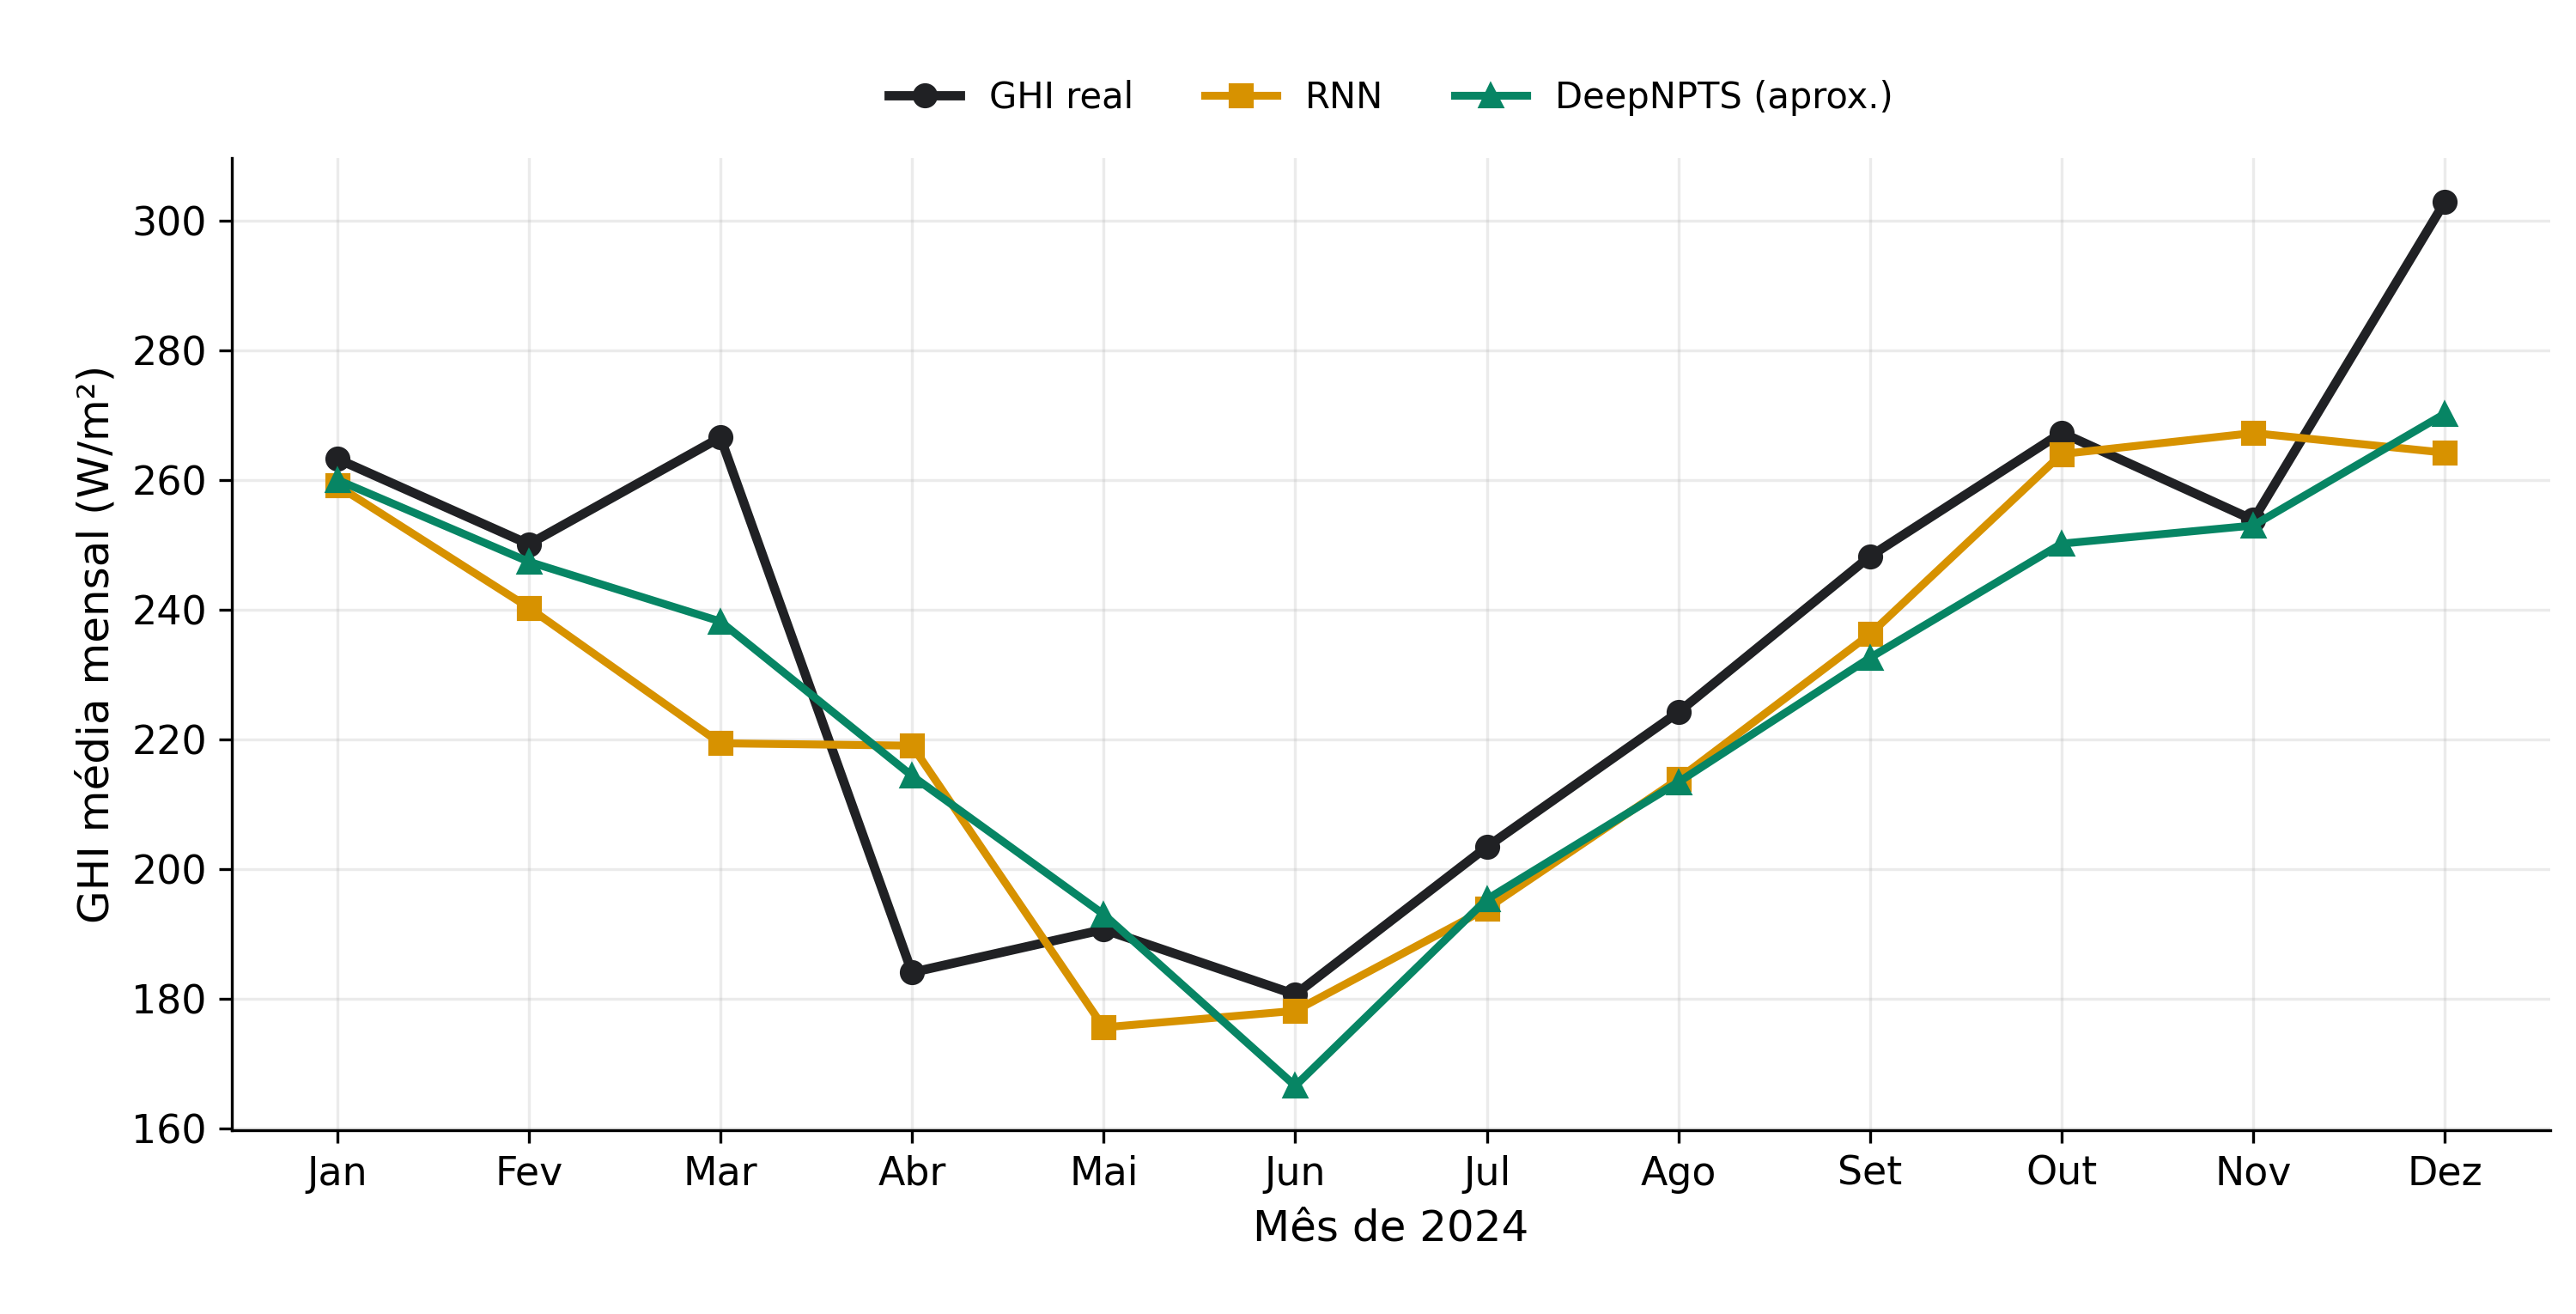
\includegraphics[width=0.90\textwidth]{figuras/previsao_mensal_byd_camacari.png}
\caption{GHI real e previsões mensais para a BYD Camaçari em 2024. A linha preta é a observação de teste; as linhas amarela e verde são, respectivamente, as previsões da RNN e da aproximação do DeepNPTS.}
\label{fig:previsao_byd}
\end{figure}

Os dois modelos reproduzem a redução da GHI no meio do ano e sua recuperação no último trimestre. A aproximação do DeepNPTS apresenta maior sobreposição com a série real em janeiro, fevereiro, maio, novembro e dezembro, enquanto a RNN é mais próxima em meses como junho e outubro. Considerando os doze pontos de teste, o MAE da aproximação foi de 13,85 W/m$^2$, contra 16,74 W/m$^2$ da RNN, correspondente a uma redução de 17,24\%. A vantagem observada decorre, portanto, do erro acumulado ao longo do horizonte de teste, e não de superioridade em todos os meses individualmente.

\section{Conclusões}
\label{sec:conclusoes}

Este trabalho avança o estudo da previsão mensal de GHI ao introduzir um sistema baseado em uma aproximação experimental do DeepNPTS para séries temporais curtas. O sistema integra aquisição e limpeza dos dados, agregação mensal, quantização, normalização, construção de atributos temporais, divisão cronológica, treinamento, avaliação e seleção pelo MAE médio entre localidades.

Na comparação global, a aproximação proposta superou os seis modelos concorrentes e foi a campeã geral, com MAE de 12,96 W/m$^2$, RMSE de 16,39 W/m$^2$, $R^2$ de 0,916 e nRMSE de 8,10\%. Em relação à RNN, melhor modelo de referência em termos médios, as reduções foram de 12,50\% no MAE e 10,07\% no RMSE. O método também venceu individualmente em cinco localidades: BMW San Luis Potosí, BYD Camaçari, Hyundai Metaplant Georgia, Rivian Normal e Tesla Gigafactory Texas. Nesta última, foi registrado o maior ganho local, com redução de 37,23\% do MAE em relação à MLP.

Os resultados indicam que a ponderação de padrões históricos por similaridade e recência constitui uma alternativa competitiva para previsão mensal de GHI. A superioridade, contudo, não foi uniforme entre localidades, e a avaliação utilizou apenas uma divisão temporal e uma execução por modelo e localidade. Consequentemente, os resultados não caracterizam a variabilidade entre diferentes inicializações ou períodos de teste. Trabalhos futuros devem incluir validação temporal em múltiplas janelas, repetições dos modelos estocásticos, horizontes superiores a um mês, variáveis meteorológicas adicionais e uma implementação canônica do DeepNPTS com treinamento conjunto de séries relacionadas.

\section*{Agradecimentos}

Os autores agradecem à FAPEMIG (processo OET-00243-26), à Universidade Estadual de Campinas (UNICAMP) e à Faculdade de Engenharia Elétrica e de Computação (FEEC) pelo apoio ao desenvolvimento deste projeto.

\begin{thebibliography}{99}

\bibitem{antonanzas2016}
J. Antonanzas et al., ``Review of photovoltaic power forecasting,'' \textit{Solar Energy}, vol. 136, pp. 78--111, 2016.

\bibitem{voyant2017}
C. Voyant et al., ``Machine learning methods for solar radiation forecasting: A review,'' \textit{Renewable Energy}, vol. 105, pp. 569--582, 2017.

\bibitem{yang2018}
D. Yang et al., ``History and trends in solar irradiance and PV power forecasting: A preliminary assessment and review using text mining,'' \textit{Solar Energy}, vol. 168, pp. 60--101, 2018.

\bibitem{duffie2013}
J. A. Duffie and W. A. Beckman, \textit{Solar Engineering of Thermal Processes}, 4th ed. Hoboken, NJ, USA: Wiley, 2013.

\bibitem{sengupta2018}
M. Sengupta et al., ``The National Solar Radiation Data Base (NSRDB),'' \textit{Renewable and Sustainable Energy Reviews}, vol. 89, pp. 51--60, 2018.

\bibitem{voyant2022}
C. Voyant et al., ``Benchmarks for solar radiation time series forecasting,'' \textit{Renewable Energy}, vol. 191, pp. 747--762, 2022.

\bibitem{sobri2018}
S. Sobri, S. Koohi-Kamali, and N. A. Rahim, ``Solar photovoltaic generation forecasting methods: A review,'' \textit{Energy Conversion and Management}, vol. 156, pp. 459--497, 2018.

\bibitem{chen2016}
T. Chen and C. Guestrin, ``XGBoost: A scalable tree boosting system,'' in \textit{Proc. 22nd ACM SIGKDD Int. Conf. Knowledge Discovery and Data Mining}, pp. 785--794, 2016.

\bibitem{hochreiter1997}
S. Hochreiter and J. Schmidhuber, ``Long short-term memory,'' \textit{Neural Computation}, vol. 9, no. 8, pp. 1735--1780, 1997.

\bibitem{chang2017}
S. Chang et al., ``Dilated recurrent neural networks,'' in \textit{Advances in Neural Information Processing Systems}, 2017.

\bibitem{salinas2017}
D. Salinas, V. Flunkert, J. Gasthaus, and T. Januschowski, ``DeepAR: Probabilistic forecasting with autoregressive recurrent networks,'' \textit{International Journal of Forecasting}, vol. 36, no. 3, pp. 1181--1191, 2020.

\bibitem{rangapuram2023}
S. S. Rangapuram et al., ``Deep non-parametric time series forecaster,'' \textit{arXiv preprint arXiv:2312.14657}, 2023.

\bibitem{nlr2026}
National Laboratory of the Rockies, ``GOES Aggregated: PSM v4 Download API,'' 2026. [Online]. Available: \url{https://developer.nlr.gov/docs/solar/nsrdb/nsrdb-GOES-aggregated-v4-0-0-download/}. Accessed: Jul. 14, 2026.

\bibitem{hyndman2006}
R. J. Hyndman and A. B. Koehler, ``Another look at measures of forecast accuracy,'' \textit{International Journal of Forecasting}, vol. 22, no. 4, pp. 679--688, 2006.

\end{thebibliography}

\end{document}
